\section{Design and Implementation of Tools}																	
\label{sec:Tools}
\vspace{\baselineskip}

\subsection{PAMEx Compiler Design and Implementation} 
\par 
\vspace{\baselineskip}
\hspace{1em}
At its core, PAMEx interprets and enforces custom, 
privileged-user-defined security information. Therefore, it was decided that it would be best to build a custom compiler to serve the purpose of defining 
PAMEx security information for several reasons. Namely, the compiler 
achieves multiple tasks at once after simply reading in an input file. 
The two primary tasks that the PAMEx compiler achieves are creating the 
output file to later be read by the File Labeler and User Database 
Builder (FLUDB) and second, to create the hierarchical level database 
to be used by PAMEx later when considering whether a given user with a given clearance has access to a given file. 
The level database can only be created by the compiler because the compiler’s 
input requires the privileged, administrative user to define all the 
levels and their relative placements. Further tools in the PAMEx system 
require all the defined levels to be written to the level database 
so that the levels can accurately be referenced and compared to.  

The PAMEx compiler was also designed for a similar purpose as many 
programming languages: to achieve its specific task in an 
efficient, flexible, and human-centric manner while clearly defining its rules \cite{levine1995}. With 
the compiler in place, the grammatical and syntactical rules are 
clearly defined so that there is no confusion about the abilities that 
PAMEx has. 
The PAMEx compiler consists of a lexer, a parser, semantic functions 
to be invoked by specific grammatical sequences found by the parser, 
and a symbol table to keep track of the variables and their corresponding 
information. The PAMEx language is not as sophisticated as many 
programming languages in the sense that it only has one scope, so the 
symbol table does not need to keep track of the scope of the variables \cite{levine2009}. For 
PAMEx’s symbol table, a hash table data structure was found to be sufficient. 

The PAMEx language grammar was originally designed using an EBNF diagram 
depicted in Figure~\ref{initalebnf} and was later revised so that it could work more easily 
with Flex and Bison as shown in Figure~\ref{yacc}. The PAMEx language file was designed to have syntax and  
grammar that is easy to understand and feel familiar to programmers. The compiler of PAMEx is used by a 
privileged user who inputs a file that both defines and assigns 
hierarchical levels and non-hierarchical labels to files and users. 
This file will further be referred to as the PAMEx language file. 
\clearpage

\begin{figure}[htb]
    \centering
    \begin{tcolorbox}[width=\textwidth, boxsep=5pt, sharp corners, colback=white, colframe=black, fontupper=\footnotesize\ttfamily] % Add a border around the lstlisting environment
        \begin{minipage}{\textwidth} % Use minipage to contain the text within the box
            \begin{lstlisting}
program ::= {component}
component ::= [comment] {definitions} [comment] {assignments} [comment]
comment ::= "#" (.)*
assignments ::= {assignment}
assignment := user-assign | file-assign
user-assign ::= "user-assign" level-name [label-list] "->" user";"
file-assign ::= "file-assign" level-name [label-list] "->" file";"
user ::= var
file ::= var
label-list ::= "[" labels "]"
labels ::= label-name{"," labels}
definitions ::= {definition}
definition ::= define-label | define-level
define-label ::= "label" label-name";"
define-level ::= "level" level-name operation";"
level-name ::= var
label-name ::= var
operation ::= "(" (setres | opvar) ")"
opvar ::= op var
setres ::= "set" res
var ::= (word | symbols) {number} {var}
symbols ::= ["." | "_" | "-"]+
number ::= [0-9]+
word ::= [A-Za-z]+
op ::= "<" | ">"
res ::= "restricted" | "unrestricted"
opt-ws ::= [WHITESPACE]+   
            \end{lstlisting}
        \end{minipage}
    \end{tcolorbox}
    \caption[EBNF Created for PAMEx]{\label{initalebnf}The Inital EBNF Diagram Created for the PAMEx Language}
\end{figure}

\clearpage

\begin{figure}[htb]
    \centering
    \begin{tcolorbox}[width=\textwidth, boxsep=5pt, sharp corners, colback=white, colframe=black, fontupper=\footnotesize\ttfamily] % Add a border around the lstlisting environment
        \begin{minipage}{\textwidth} % Use minipage to contain the text within the box
            \begin{lstlisting}
%%

stmt_list   : 	stmt_list stmt
            |	stmt {};
stmt        :	USERASSIGN level_name ASSIGN user`;' { ... }
            |	USERASSIGN level_name label_list ASSIGN user`;'	{ ... }
            |	USERASSIGN label_list ASSIGN user`;' { ... }
            |	FILEASSIGN level_name ASSIGN file`;' { ... }
            |   FILEASSIGN level_name label_list ASSIGN file`;' { ... }
            |	FILEASSIGN label_list ASSIGN file`;' { ... }
            |	LABEL label_name`;' { ... }
            |	LEVEL level_name op`;' { ... };
label_list  :	`['labels`]' { ... };
labels      :	label_name  { ... }
            |	label_name`,' labels { ... };	
user        :	id { $$ = $1; };
file        :	id { $$ = $1; };
level_name  :	id { $$ = $1; };
label_name  :	id { $$ = $1; };	
op          :	`('set_res`)' { $$ = $2; }
            |	`('op_var`)' { $$ = $2; };	
op_var      :	CMP id { ... };
set_res     :	SET res { ... };
res         :	LEVELLIT { $$ = $1; };
id          : 	ID { $$ = $1; };

%%
            \end{lstlisting}
        \end{minipage}
    \end{tcolorbox}
    \caption[Code Snippet from PAMEx Yacc File]{\label{yacc}A Partial Code Snippet Taken from PAMEx's Yacc File Depicting the PAMEx Grammar. Semantic Functions have been Omitted.}
\end{figure}

\vspace{\baselineskip}

\subsection{PAMEx Language File Design}
\par 
\vspace{\baselineskip}
\hspace{1em}
Syntactically, the PAMEx language file was designed with two distinct 
actions in mind: defining the PAMEx security information and assigning 
the security to users and files. The definition actions would allow the 
privileged user to define the hierarchical levels including the levels’ 
names and what placement they are in the hierarchical chain in relation 
to other levels. Labels on the other hand, are 
compartments and are standalone qualifications that do not have any 
hierarchical value \cite{natsecinfo}. Therefore, the only information that a privileged 
user needs to provide when defining a new label is its name. Designing 
the PAMEx language file syntax and grammar to be user-friendly was an 
important consideration. Therefore, the definitions 
section’s syntax and grammar are inspired by many programming languages by 
consisting of a keyword to be used as a type, a variable name, an 
operation for level definitions, and a semi-colon to mark the end of 
the statement. For example, in PAMEX, a level definition followed by a label 
definition might look like the following two lines. 

\begin{verbatim}
level administrator (> developer); 
label alpha; 
\end{verbatim}

For the assignment statements, the PAMEx language file depicts 
which level and labels are assigned to users and files. At any 
point, any user and any file may only be assigned one level to have a 
distinguished security group but may have zero or more labels to 
further define the security assigned. Assignment statements were 
designed to be minimalistic, easy to read, and also resemble that of other 
programming languages. The grammar for an assignment statement 
includes the function to be performed, the name of the level to assign 
to the entity, the list of labels to assign, an assignment operator, 
the name of the entity, and finally a semi-colon to depict the end of 
the statement. For our previous example with the technology company, 
the \texttt{administrator} Alice and \texttt{alpha}\texttt{\_dev}\texttt{\_instructions.txt} could be assigned
to the system using PAMEx with the following lines. 

\begin{verbatim}
user-assign administrator [alpha, beta, charlie] -> Alice; 
file-assign developer [alpha] -> alpha_dev_instructions.txt; 
\end{verbatim}

From these assignment statements, Alice would be assigned the level \texttt{administrator} and the labels 
of \texttt{alpha}, \texttt{beta}, and \texttt{charlie}. \texttt{alpha}\texttt{\_dev}\texttt{\_instructions.txt} would be assigned the level 
\texttt{developer} and the label \texttt{alpha}.  

The division of the definition and assignment statements in the PAMEx 
language file is not a hard one. Much 
like many programming languages, definitions and assignments are 
allowed to be intermixed throughout the PAMEx language 
file with the only grammatical requirement of a level or a label 
needing to be defined before it can be assigned to a user or a file. 
With this qualification in mind, our complete 
PAMEx language file example with the user Alice and \texttt{alpha}\texttt{\_dev}\texttt{\_instructions.txt} could 
look like Figure~\ref{languageex}. 
\clearpage

\begin{figure}[htb]
    \centering
    \begin{tcolorbox}[width=\textwidth, boxsep=5pt, sharp corners, colback=white, colframe=black, fontupper=\footnotesize\ttfamily] % Add a border around the lstlisting environment
        \begin{minipage}{\textwidth} % Use minipage to contain the text within the box
            \begin{lstlisting}
# This is a comment 
# alpha_dev_instructions.txt and Alice example 

# Definitions for alpha_dev_instructions.txt 
level public (set unrestricted);
level general_staff (set restricted); 
level developer (> general_staff); 
label alpha; 
label beta; 

# Assignment of security for alpha_dev_instructions.txt 
file-assign developer [alpha] -> alpha_dev_instructions.txt;

# Further definitions for Alice 
level administrator (> developer);
level executive_staff (> administrator);
label charlie; 

# Assignment of security for Alice 
user-assign administrator [alpha, beta, charlie] -> Alice;
            \end{lstlisting}
        \end{minipage}
    \end{tcolorbox}
    \caption[Full, Simple PAMEx Language File Example]{\label{languageex}A Full Example of the PAMEx Language File Contents with User Alice and alpha\_dev\_instructions.txt}
\end{figure}

One of the major decisions that had to be made when designing the PAMEx language file was how the 
level placements could be defined syntactically and grammatically. In 
PAMEx, levels are a tiered, hierarchical system and therefore, it was decided that it would make sense for the levels to be defined 
in relation to one another. For example, a PAMEx language file could be written so that a level defined with the name 
\texttt{general\_staff} is a lower placement than a level defined with the name 
\texttt{developer}, which is a lower placement than a level named \texttt{administrator}. 
For the privileged user to define levels relationally, a base level needed to be defined first – a level whose hierarchical placement is set independently 
rather than relationally. Therefore, the PAMEx language file allows for three different operations: the first being the 
operation \texttt{set} which allows a level to be set to a base level of either 
\texttt{unrestricted} which is hierarchical placement zero or \texttt{restricted} which is 
hierarchical placement one, as well as the operations \texttt{$>$} and \texttt{$<$} which 
define that a level is either one hierarchical placement greater than 
a previously defined level or one hierarchal placement less than a 
previously defined level.  

Another major development decision was that no two levels would share a 
hierarchical placement. In other words, if there are three levels \texttt{a}, 
\texttt{b}, and \texttt{c} they could be defined as the following lines. 

\begin{verbatim}
level a (set restricted); 
level b (> a); 
level c (< b); 
\end{verbatim}


Before level \texttt{c} is defined, level \texttt{b} is one hierarchical placement higher 
than level \texttt{a}. This is because level \texttt{b} is defined using the $>$ 
operation to depict that level \texttt{b} is one placement higher than level \texttt{a} 
in the hierarchy. On the next line, when level \texttt{c} is defined as one 
placement less than level \texttt{b} using the $<$ operation, level \texttt{c} does not take the same placement as 
level \texttt{a}, but rather the level placement of \texttt{b} shifts and makes room for 
the new level. Therefore, the level placement order in this scenario 
would be first, at the lowest level placement, level \texttt{a}, then one 
placement higher is level \texttt{c}, then, with the highest-level placement, 
level \texttt{b}. 

With this relational method, the privileged user can easily 
and clearly define a hierarchical level structure using PAMEx, and the 
grammar is designed in such a way that is easy to interpret. The language file is also minimal in the 
sense that each character sequence in the grammar has a purpose, but it 
is powerful in the sense that the security can be defined to meet many 
systems' needs. 

The PAMEx compiler is also convenient in the sense that not all users and 
files on the system need to be assigned PAMEx security clearance 
information. For any user or file that is not deliberately assigned a 
level, the level of the file or user is treated as a level at placement 
zero or \texttt{unrestricted}. In other words, if a file is not assigned a level, 
then PAMEx does not affect the access that a user has to the file. If a 
user is not assigned a level, they cannot access any PAMEx secured file 
that has a level higher than the set placement of \texttt{unrestricted}. This 
was an important decision to allow for PAMEx to work 
with already defined security policies on a system and to allow PAMEx 
to work out of the box for the privileged administrative user to only 
worry about defining the security policies for those users and files 
that it will affect. 

Another notable point of flexibility with the PAMEx compiler is when 
assigning security information to files. Within the assignment 
statement, the file specified does not need to be simply the name of a 
file but can instead be the path to a file. This path is relative to a 
directory specified when using the FLUDB tool. Being able to specify the 
path to a file at this stage gives the privileged administrative user the ability 
to enforce a PAMEx security policy in multiple locations on the system. 
\vspace{\baselineskip}

\subsection{The PAMEx Compiler Outputs Two Files: The Assignments File and a Level Database} \label{policy-out}
\par 
\vspace{\baselineskip}
\hspace{1em}
When the compiler runs successfully, an output file is created containing all 
the user and file assignment information. This file is written in such a 
way that the computer will be able to easily read and interpret it, but is also relatively simple for a human to read because 
there is an evident pattern in the format. For our running example of 
\texttt{alpha}\texttt{\_dev}\texttt{\_instructions.txt} and user Alice, the PAMEx compiler output may look like
the example in Figure~\ref{compout}.
\clearpage

\begin{figure}[htb]
    \centering
    \begin{tcolorbox}[width=.8\textwidth, boxsep=5pt, sharp corners, colback=white, colframe=black, fontupper=\footnotesize\ttfamily] % Add a border around the lstlisting environment
        \begin{minipage}{\textwidth} % Use minipage to contain the text within the box
            \begin{lstlisting}
FILE_LEVEL alpha_dev_instructions.txt developer:2 
FILE_LABELS alpha_dev_instructions.txt alpha 
USER_LEVEL Alice administrator:3 
USER_LABELS Alice alpha 
USER_LABELS Alice beta 
USER_LABELS Alice charlie 
            \end{lstlisting}
        \end{minipage}
    \end{tcolorbox}
    \caption[PAMEx Compiler Output File Example]{\label{compout}An Example of a PAMEx Compiler Output File with User Alice and alpha\_dev\_instructions.txt}
\end{figure}

Each line depicts an assignment function that should occur. For example,
the first line has the \texttt{FILE\_LEVEL} keyword to depict that a file is to 
be assigned a level, then the path to the file, and finally, the level 
information including the name and its placement in the hierarchy 
separated by a colon delimiter. The level placement number is 
unnecessary for further functionality because all level information 
including their placement numbers are stored in the level database. 
The level placement numbers in the compiler output file are 
simply present as extra data for debugging and development purposes. 
When developing the FLUDB tool for instance, the level placements 
were used to compare and double check that the tool was gathering the 
appropriate level data. 

In addition to the policy-out file, the PAMEx compiler outputs a level 
database file. The level database file was created because there is a 
need to compare the placement of two levels in future tools. The 
placement comparison was found to be most reliable if the level 
information persisted in one place on the system. It is essential to output the level database file at this 
stage because the PAMEx language file is the only place where all the 
levels are defined and ordered by placement. The levels are developed 
to be compared relationally and therefore it is necessary that every 
level is accounted for in some way. The levels database therefore 
captures a list of all the levels that have been defined in the PAMEx 
language file in hierarchical order. Each line of the level database 
file contains a level name and its placement number separated by a 
colon delimiter. For our running example of the technology company, the level database file could look like 
the example in Figure~\ref{leveldb}.
\clearpage

\begin{figure}[htb]
    \centering
    \begin{tcolorbox}[width=.3\textwidth, boxsep=5pt, sharp corners, colback=white, colframe=black, fontupper=\footnotesize\ttfamily] % Add a border around the lstlisting environment
        \begin{minipage}{\textwidth} % Use minipage to contain the text within the box
            \begin{lstlisting}
public:0
general_staff:1
developer:2
administrator:3
executive_staff:4
            \end{lstlisting}
        \end{minipage}
    \end{tcolorbox}
    \caption[PAMEx Level Database Example]{\label{leveldb}An Example of the Contents a PAMEx Level Database Outputted by the FLUDB Tool}
\end{figure}


\vspace{\baselineskip}

\subsection{Design and Implementation of The File Labeler and User Database Builder (FLUDB) Tool}
\par 
\vspace{\baselineskip}
\hspace{1em}
It was determined from the beginning that a tool would need to be 
created to interpret the compiler’s output and pass along the 
information given. The tool could do this by labeling the files with 
their respective security information and by creating a database file 
containing the system users’ PAMEx security information. Therefore, the 
File Labeler and User Database Builder (FLUDB) tool was designed and 
created in C for PAMEx to do just that. To work flexibly, the FLUDB 
tool would need initial information pertaining to the locations of the 
input and output files. Therefore, the tool takes three input 
parameters from the administrative user which are as follows: the path to the compiler-created 
policy-out file, the directory that houses the files specified in 
policy-out which will be assigned the PAMEx security levels and labels, 
and the path for the targeted users database output file. The PAMEx 
FLUDB tool is limited in the way that all the files that are defined 
in the PAMEx language file need to be in the same directory or share a 
parent directory. The benefit to keeping all the PAMEx restricted 
files in one location are that the interpreter does not need to search 
through an entire file system to find the correct file, but only search
for files that are within the specified parent directory.

One of the first hurdles that was faced during the development of the 
FLUDB tool was determining how to store the file’s PAMEx security 
information including the file’s level and various labels. To overcome this hurdle Linux security modules were studied, namely SELinux. 
It was found that SELinux uses a file property called extended 
attributes \cite{selinux}, so PAMEx followed suit. Extended attributes are a metadata 
feature of a filesystem that are built into many operating systems. 
They are lightweight features that allow for key-value pairs pertaining 
to a file’s information and unlike most file metadata, extended 
attributes are not interpreted by the files themselves, but rather by 
outside programs. For those reasons extended attributes are a perfect 
system to store security information. Each file and directory on a Unix 
system has extended attributes so therefore any particular file can 
hold information about its own security \cite{man7xattr}.   

Further inspired by SELinux, the C 
programming language’s \texttt{xattr} library was found and utilized to achieve all extended 
attribute operations. Particularly, the PAMEx FLUDB tool uses the 
\texttt{setxattr} function to set both the key and the value of the extended 
attributes for both levels and labels on a file. The \texttt{setxattr} function 
requires root privileges and therefore the FLUDB tool needs to be run 
as \texttt{root} to write the files’ security information \cite{man7xattr}. Although at first 
seen as a drawback, being required to run the FLUDB tool 
as \texttt{root} is useful in the sense of providing an extra layer of security 
in order for PAMEx levels and labels to be assigned to files on a 
system. In other words, the files cannot have security restrictions be 
added to them if the FLUDB tool cannot write to the file’s extended 
attributes and the only users able to use the FLUDB tool are those with \texttt{root} access.  

For the design of the extended attributes themselves, two different extended attributes were created for each file pertaining to 
PAMEx security information. One of the extended attributes is for the 
file’s PAMEx level with the key \texttt{security.fsc.level} and the other is for 
the list of the file’s PAMEx labels with the key \texttt{security.fsc.label}. 
The policy-out file which contains the information to write to the two 
extended attributes is written in such a way that the file assignment 
information is provided on separate lines but grouped together. Looking
again at Figure~\ref{compout} all the \texttt{alpha}\texttt{\_dev}\texttt{\_instructions.txt}
assignment statements are grouped together and all of the assignment statements
for Alice are grouped together.

Grouping the data in policy-out is a purposeful feature so that the 
file’s attributes can be interpreted more efficiently. When the FLUDB tool reads 
a line that begins with \texttt{FILE\_LEVEL}, it knows to assign or reassign 
a value to the extended attribute with the key \texttt{security.fsc.level} to the 
file specified. The value of the extended attribute is the remaining
information in the same policy-out file line including the 
level’s name and its placement. When the FLUDB tool reads a line that 
begins with \texttt{FILE\_LABELS} it knows to append a new label to the value of 
the file’s extended attribute with the key \texttt{security.fsc.labels}. The 
interpreter will read the rest of the line which will give the FLUDB 
tool the file to assign the label to, and then the label name. If the 
file is to be assigned more than one label, the following sequential 
lines will contain the additional labels. Figure~\ref{xattrex} is 
an example of a file’s extended attributes after the FLUDB file has 
written its security information.

\begin{figure}[htb]
    \centering
    \begin{tcolorbox}[width=.8\textwidth, boxsep=5pt, sharp corners, colback=white, colframe=black, fontupper=\footnotesize\ttfamily] % Add a border around the lstlisting environment
        \begin{minipage}{\textwidth} % Use minipage to contain the text within the box
            \begin{lstlisting}
# file: alpha_dev_instructions.txt
security.fsc.labels="alpha"
security.fsc.level="developer:2"
security.selinux="unconfined_u:object_r:user_tmp_t:s0"
            \end{lstlisting}
        \end{minipage}
    \end{tcolorbox}
    \caption[Example of Extended Attributes Written by PAMEx]{\label{xattrex}An Example of alpha\_dev\_instructions.txt's Extended Attributes After Being Processed with PAMEx}
\end{figure}

From this example, PAMEx's security information is evident in \texttt{alpha}\texttt{\_dev}\texttt{\_instructions .txt}'s
extended attributes. The first line depicts a definition of the file being
accessed, and the second and third lines show the extended attributes written
by PAMEx. The first of which are \texttt{alpha}\texttt{\_dev}\texttt{\_instructions.txt}'s PAMEx labels with the key of
\texttt{security.fsc.labels} and the value of \texttt{alpha}\texttt{\_dev}\texttt{\_instructions.txt}'s list of labels assigned to
it delimited by a colon. Similarly, the next line depicts \texttt{alpha}\texttt{\_dev}\texttt{\_instructions.txt}'s level
information with the key of \texttt{security.fsc.level} and value of the level name
and level placement delimited by a colon. The last line pertains to security
information invoked by SELinux, and is thus orthogonal to PAMEx.

Through the process of invoking error handling, it was ensured that if an error is to occur while invoking a 
function from the xattr library, the appropriate error label would be 
printed. This feature is especially useful when the privileged user is 
unaware or forgets that the FLUDB tool needs to run as root. 

The user database is created by the FLUDB tool alongside the 
extended attribute assignments. While reading the policy-out file line 
by line, the FLUDB tool may come across two different user actions to 
perform: \texttt{USER\_LEVEL} and \texttt{USER\_LABELS} respectively. Much like the 
interpreted file lines, the user lines were also created to be 
standalone actions. This means that the user information can be written 
in any order anywhere in the file and FLUDB will still be 
able to correctly interpret it. In addition to the reasons stated 
above regarding the interpreted file lines, the dynamism of the 
FLUDB tool also allows for fewer bugs and greater flexibility. 

Figure~\ref{usersdbex} depicts an example of an extended users database with our 
working example of the administrator Alice and developer Bob.

\begin{figure}[htb]
    \centering
    \begin{tcolorbox}[width=.8\textwidth, boxsep=5pt, sharp corners, colback=white, colframe=black, fontupper=\footnotesize\ttfamily] % Add a border around the lstlisting environment
        \begin{minipage}{\textwidth} % Use minipage to contain the text within the box
            \begin{lstlisting}
Alice:administrator:3:alpha:beta:charlie 
Bob:developer:2:beta:charlie 
            \end{lstlisting}
        \end{minipage}
    \end{tcolorbox}
    \caption[Example of PAMEx Targeted Users Database Contents]{\label{usersdbex}The Contents of an Example Targeted Users Database Written by PAMEx}
\end{figure}

\vspace{\baselineskip}

\subsection{Design and Implementation of PAMEx's Pluggable Authentication Module (PAM)}
\par 
\vspace{\baselineskip}
\hspace{1em}
The final tool that needed to be designed to implement the bare 
functionality of PAMEx was the PAM module. With the implementation of 
the FLUDB tool, PAMEx has a method of creating a targeted users 
database which holds all the system users’ PAMEx security information 
and a way to write all the files’ extended attributes which labels 
files with security information. The next step is the ability for the 
system to know who is logged in and for the system to have the 
necessary information on hand when checking the security clearance of a 
user. In its end state, PAMEx should be able to cross reference a 
user’s security information with a file’s extended attributes to 
determine if a user has the proper security clearance to access said 
file. For this to occur, the system must know who the logged in user is 
and therefore, store their PAMEx security information during a system user's authentication \cite{lauber}. 
In our example, when the user Alice logs in to the system, the 
system will need to know what level of PAMEx security clearance Alice 
has access to and what security labels Alice has access to. 
Attention was turned once again to preexisting Linux Security 
Modules including SELinux \cite{selinux}. It was determined that the best way to 
achieve the functionality needed was through the use of a PAM module.  

PAM separates authentication and user session functionality into 
different modules. The modules are stacked on top of each other and 
performed as steps in an authentication process. The steps are sorted into two 
types: authentication modules and session modules. Authentication 
modules are performed during the authentication of a user, and session 
modules are performed after the authentication of a user and during 
that user’s session on the system. Therefore, when a user authenticates 
onto a system, a particular set of PAM modules are invoked depending on 
where and how the user authenticated \cite{lauber}. While relatively simple from a 
high perspective, PAM modules are complicated to develop and can be 
dangerous to a system if invoked improperly. Many issues can occur if 
a user incorrectly invokes a PAM module, but most likely, the system’s 
user login process will fail due to an error. The error often breaks 
the login system and further forbids a user from logging in. At this 
stage, development was continued on a virtual machine 
to ensure the safety of the system.

PAM C libraries were used to create the PAM module \cite{man7pam}. In the C library, PAM 
module actions are divided into categories such as authenticate, open session, 
close session, or manage account. For PAMEx, the only action that needs 
to be involved is the authenticate action. This is because PAMEx’s PAM 
module creates and stores stagnant user information upon successful 
authentication of a system user which does not need to be modified 
during a user’s session on the system. PAMEx’s PAM module was developed 
as a shared object file type and placed in the \texttt{/lib64/security} 
directory much like the other PAM modules installed on the system so that it can be later accessed by PAM configuration files. 
The custom-developed module is invoked as the first 
action in the \texttt{system-auth} and \texttt{password-auth} PAM configuration files found in 
\texttt{/etc/pam.d}. Figure~\ref{system-auth} depicts the first few PAM authentication 
processes of the \texttt{system-auth} file found in \texttt{/etc/pam.d} including PAMEx's PAM module \texttt{pam\_pamex.so}. 
\texttt{system-auth} and \texttt{password-auth} are invoked every time a user graphically 
logs into the system, when a user uses the \texttt{su} command to log into a 
kernel on the system, and when \texttt{sudo} is used \cite{lauber}.

\begin{figure}[h]
    \centering
    \begin{tcolorbox}[width=\textwidth, boxsep=5pt, sharp corners, colback=white, colframe=black, fontupper=\footnotesize\ttfamily] % Add a border around the lstlisting environment
        \begin{minipage}{\textwidth} % Use minipage to contain the text within the box
            \begin{lstlisting}
# Generated by authselect on Wed Jan 18 20:28:10 2023
# Do not modify this file manually, use authselect instead. 
# Any user changes will be overwritten.
# You can stop authselect from managing your configuration by calling 
# 'authselect opt-out'.
# See authselect(8) for more details.

auth    required                        pam_pamx.so /etc/userdb /tmp
auth    required                        pam_env.so
auth    required                        pam_faildelay.so delay=2000000
auth    sufficient                           pam_fprintd.so
auth    [default=1 ignore=ignore success=ok] pam_usertype.so isregular
auth    [default=1 ignore=ignore success=ok] pam_localuser.so
auth    sufficient                           pam_unix.so nullok
auth    [default=1 ignore=ignore success=ok] pam_usertype.so isregular
auth    sufficient                           pam_sss.so forward_pass
auth    required                             pam_deny.so
                
            \end{lstlisting}
        \end{minipage}
    \end{tcolorbox}
    \caption[Code Snippet from system-auth File]{\label{system-auth}Code Snippet Pulled from System-Auth Depicting Implementation of PAMEx's PAM Module}
\end{figure}

Figure~\ref{PAM Diagram} depicts how PAM modules are invoked on a system with PAMEx via various authentication processes.
When a system user authentication process occurs, the corresponding PAM configuration files are invoked where various PAM
modules are performed in succession.

\begin{figure}[h]
\centering
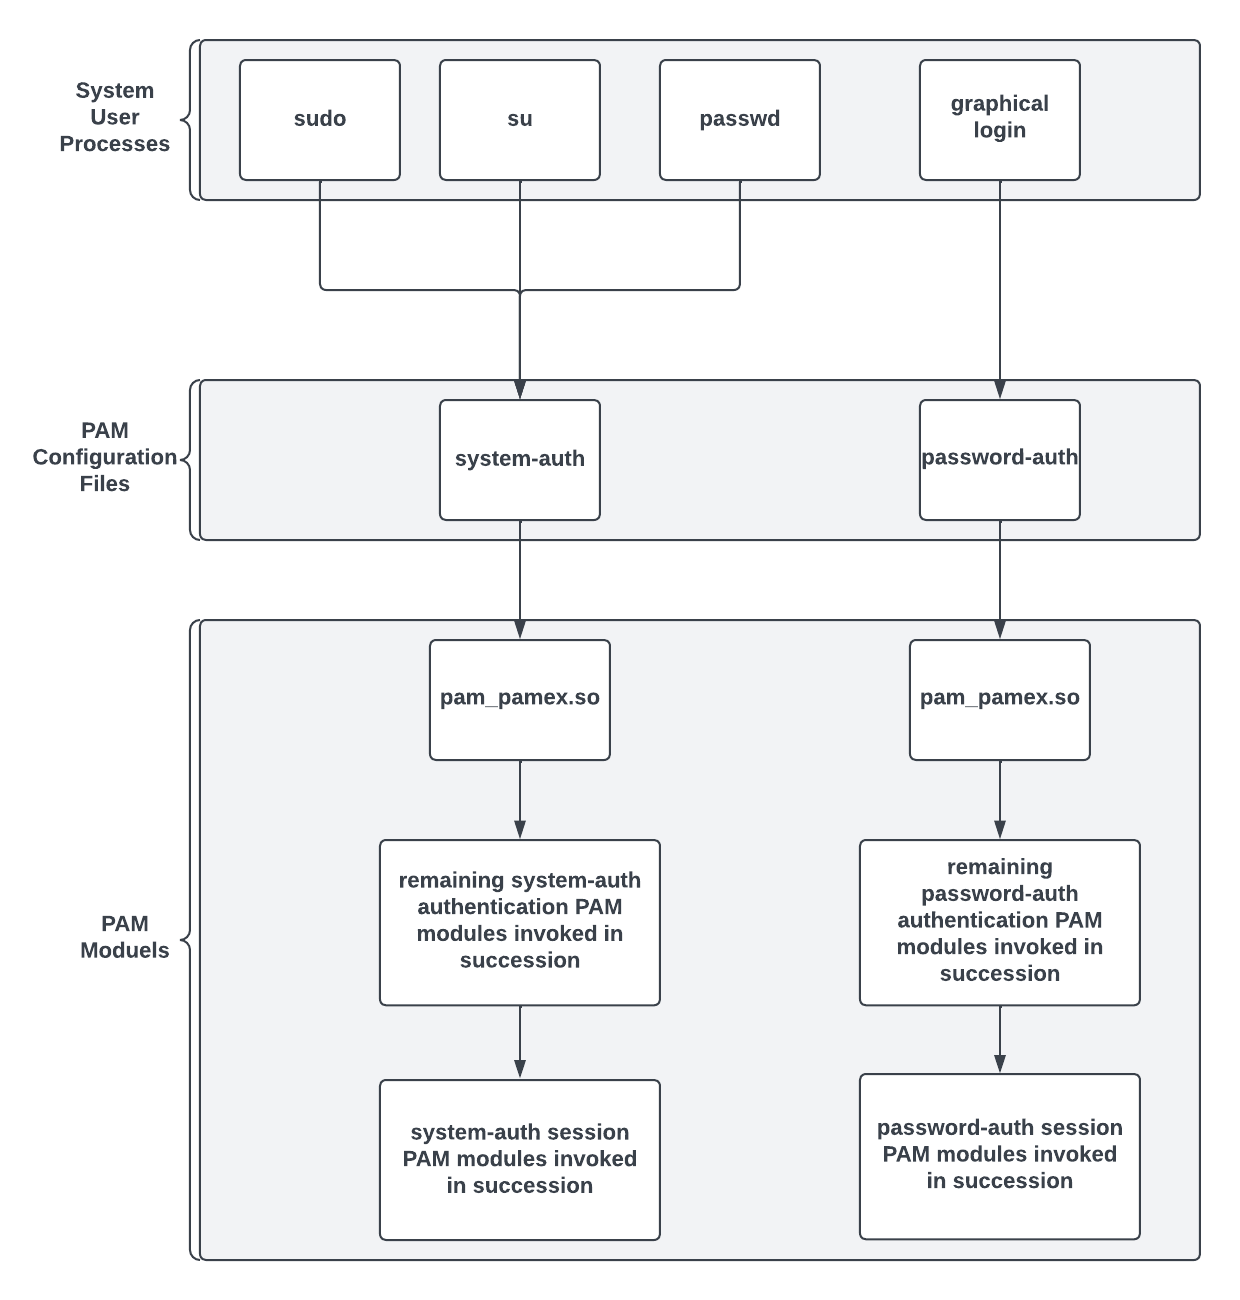
\includegraphics[width=.9\textwidth]{section04/assets/pam_overview.png}
\caption[Overview of PAM Modules on PAMEx]{\label{PAM Diagram}Overview of PAM Modules on PAMEx}
\end{figure}

Authenticating on a system using any of the above methods invokes PAMEx’s 
custom PAM module and creates an information file that mimics the file 
which Linux Security Modules such as SELinux create upon user 
authentication. SELinux’s informational file is named current and is 
located at \texttt{/proc/$<$pid$>$/attr} where \texttt{$<$pid$>$} is replaced with the process 
ID of the authentication process \cite{selinux}. The process is forked as a child from the 
authentication process and any subsequent processes that the user invokes will be children to
that process. The idea is that the signed-in user's PAMEx security information will be available
through their session on the system.

A shortcoming of PAMEx is that 
its PAM module is unable to write to the system process file directory, 
\texttt{proc}. On most systems with this security method, the \texttt{proc} directory 
has write restrictions to disallow a user from being able to write ill-formed data,
and the current kernel requires an SELinux format. While lacking a custom kernel 
that would allow write access to process files, the PAMEx PAM module 
uses a work around by creating a fake, mimicked output process file 
which holds the logged in user’s PAMEx security information that it 
would otherwise hold in the \texttt{proc} directory which the system calls 
pseudo-proc. The fake file can be outputted to any writable location. 
The following line depicts an example of what the pseudo-proc file contents might look like with our 
working example of the system user Alice. 

\begin{verbatim}
Alice:top_secret:3:alpha:beta:charlie
\end{verbatim}

\vspace{\baselineskip}

\subsection{Design and Implementation of the Extraneous File Labeler Tool}
\par 
\vspace{\baselineskip}
\hspace{1em}
After creating the PAM module for PAMEx, it was quickly realized 
that there was an optimization issue that had a simple solution. The 
issue was that in the common scenario that a privileged, administrative 
user wanted to change the specification of the PAMEx security of a file 
after the security definitions had been assigned, the privileged user 
would need to re-write the PAMEx language file and run it through both 
the parser and the interpreter again. This two-step process could 
instead be handled in one after a security policy had previously been defined on a system and 
therefore, the Extraneous File Labeler tool was developed.  

The File Labeler tool’s job is to conform to the previously defined 
PAMEx security information but allow a privileged user to add, update, 
or remove a security level or label to a file. The File Labeler tool is 
a simple C script that takes in four arguments regarding how the 
privileged user is to change a file’s security information. The first 
argument is the path to the level database that has already been 
created by the PAMEx parser. Any level that the privileged user 
redefines must come from the level database specified. The second 
argument is the path to the file whose security information is being 
changed. The third argument is a flag which specifies what process is 
to be done to the specified file including \texttt{ -al -cl -dl} for add level, 
change level, and delete level respectively and \texttt{ -ac -rc} 
for add label 
and remove label respectively. The last argument that the File Labeler 
takes in is a level or label name. In the case of removal, this name 
must match an already defined level or label in the file’s extended 
attributes, but in the case of a change or addition, the name may be 
unique to the file so long that, in the case that a level is being 
added or changed, the level is contained in the level database. For 
example, if we wanted to change the level of \texttt{alpha}\texttt{\_dev}\texttt{\_instructions.txt} from \texttt{developer} to 
\texttt{general\_staff}, a privileged user could use the File Labeler tool with the 
command below. 

\begin{verbatim}
./file-labeler ../data/level-database 
    ../files/alpha_dev_instructions.txt -cl general_staff
\end{verbatim}

Figure~\ref{xattrmod} depicts \texttt{alpha}\texttt{\_dev}\texttt{\_instructions.txt}'s 
exteded attributes after the above command has modified \texttt{alpha}\texttt{\_dev}\texttt{\_instructions.txt}.

\begin{figure}[htb]
    \centering
    \begin{tcolorbox}[width=.8\textwidth, boxsep=5pt, sharp corners, colback=white, colframe=black, fontupper=\footnotesize\ttfamily] % Add a border around the lstlisting environment
        \begin{minipage}{\textwidth} % Use minipage to contain the text within the box
            \begin{lstlisting}
# file: alpha_dev_instructions.txt
security.fsc.labels="alpha"
security.fsc.level="general_staff:1"
security.selinux="unconfined_u:object_r:user_tmp_t:s0"
            \end{lstlisting}
        \end{minipage}
    \end{tcolorbox}
    \caption[Extended Attributes After Being Modified by PAMEx's Extraneous File Labeler Tool]{\label{xattrmod}An Example of alpha\_dev\_instructions.txt's Extended Attributes After Being Modified by PAMEx's Extraneous File Labeler Tool}
\end{figure}

\vspace{\baselineskip}

\subsection{Design and Implementation of the Oracle Tool}
\par 
\vspace{\baselineskip}
\hspace{1em}
A Linux kernel can enforce Linux security modules to affect how the kernel imposes its access controls.
For a Linux security module, the kernel is written in such a way that 
allows for the module to perform its actions because of specific 
commands running \cite{kerneldocs}. PAMEx does not yet provide a Linux security module. 
It was decided to omit the development of a custom kernel because of the 
major challenge and it holds which is a challenge that is not needed to demonstrate the  
functionality of the PAMEx tool suite. The task of creating a custom 
kernel in addition to the PAMEx compiler and tool suite would have also 
greatly extended the PAMEx project’s development time.  

In lieu of the customized kernel, a tool called 
Oracle was created that allows a user to check if a logged-in system user has the 
PAMEx security clearance to access a particular file. Oracle is a 
user-prompt tool where the user submits queries about the PAMEx 
security of a system including the signed in user’s PAMEx user security 
information, a file’s PAMEx security information and whether the signed 
in user has the PAMEx security clearance needed to access a file. 
Oracle’s primary function is to cross-check a file’s extended 
attributes related to PAMEx with the process file that PAMEx’s PAM 
module created containing the signed in user’s information. With the 
use of this information, Oracle can inform the user if the signed in 
user has access to the specified file, and if not, why? 

After a user authenticates on a system, PAMEx's PAM module creates a fake
process file with user information as mentioned in Section 3.5.
This is a replacement to how a custom kernel would propagate a process
to be forked as a child from the authentication process. 
The way that Oracle works is it first prompts the user for the fake 
process ID that the PAMEx PAM module creates the directory for. The 
Oracle user inputs the fake process file ID and if it is found, Oracle then 
allows the user to input a command to find out more about the 
authenticated user or a file’s PAMEx security information.  

Oracle was by no means developed to be a replacement to a custom 
kernel. Instead, Oracle serves as an end-to-end simulation that brings 
together and demonstrates all the PAMEx tools and components. Oracle 
allows a PAMEx user to effectively demonstrate all PAMEx’s functionality 
in a working environment. Figure~\ref{oracle} depicts Oracle working
and demonstrating the full functionality of PAMEx.
\clearpage

\begin{figure}[htb]
    \centering
    \begin{tcolorbox}[width=\textwidth, boxsep=5pt, sharp corners, colback=white, colframe=black, fontupper=\footnotesize\ttfamily] % Add a border around the lstlisting environment
        \begin{minipage}{\textwidth} % Use minipage to contain the text within the box
            \begin{lstlisting}
Welcome to the PamEx Oracle!
Enter PID
    > 4571

Pid accepted.

Type help for a list of commands.
    > help

Pamx Oracle Commands:
help - print list of commands
user - check the name of the signed in user
userinfo - get the name and security information of signed in user
checkfileaccess - check if the signed in user can access a file
cfa - alias for the checkfileaccess command
fileinfo - get the authentication information of a file
quit - quit the Oracle

    > cfa

File path: ../tests/assignment_files/alpha_dev_instructions.txt

Access denied. User level too low.
            \end{lstlisting}
        \end{minipage}
    \end{tcolorbox}
    \caption[Oracle Tool Demonstration]{\label{oracle}A Working Example of the Oracle Tool Being Used}
\end{figure}

\vspace{\baselineskip}

% \subsection{The Omission of a Custom Kernel}
% \par 
% \vspace{\baselineskip}
% \hspace{1em}
% The most important component that is omitted from the PAMEx system is a 
% customized Kernel. Among other tasks, the Kernel’s role in the system 
% would be to observe all the PAMEx security data to officiate which user 
% invoked processes are allowed as further explained in Section 3.5. The idea is that processes that are used 
% to access the file will be branched from the process that was used to 
% authenticate the user. Since the authentication process uses a PAM 
% module to automatically write the authenticated user’s PAMEx security 
% clearance information, the kernel can check the user’s clearance 
% information to see if they are allowed to perform processes to access 
% the file. Therefore, whenever a user attempts to access a file, their 
% PAMEx credentials are cross checked with the file’s extended attributes 
% which tells the kernel if the user has access or not \cite{kerneldocs}. Continuing with our
% technology company example, if the developer Bob has a PAMEx level clearance of \texttt{developer} 
% and there is a file called \texttt{password\_file.txt} on the same system with a 
% PAMEx clearance level of \texttt{administrator}. While Bob is authenticated on the 
% system, if he uses the process \texttt{cat} to try to view \texttt{password\_file.txt}’s 
% contents, the kernel will recognize the command \texttt{cat} as a command used 
% to access file information, determine that Bob does not have the 
% credentials to access the file, and stop the \texttt{cat} process 
% from running. Section 3.7 explains how the Oracle tool gets around this issue.

% Another major reason for implementing a custom kernel is to be able to 
% properly store the user information within the running process’ data 
% in the first place. When a process is running on Linux, a directory for 
% that process is created in the \texttt{proc} directory named after the process’ 
% ID. For instance, if a C process in ran called \texttt{foo} with a process ID of 
% 12345, there will be a directory named 12345 in the \texttt{proc} directory 
% containing data for that process \cite{kerneldocs}. It is within a \texttt{proc} directory that 
% the authenticated user security information should be written. For 
% example, SELinux creates files containing user security information in 
% a file with the path \texttt{proc/<process\_id>/attr/current} \cite{selinux}. The major drawback 
% to writing proc files this way though is that these files may not be 
% edited by non-root processes and when attempting to do so the system throws a error, so a 
% custom kernel must be created to write to the \texttt{proc} file. 

% Overall, the omission of the kernel means that PAMEx cannot function as an independent
% Linux security module. PAMEx is still able to fully show an end-to-end implementation
% of being a security tool suite without the custom kernel though.

% \vspace{\baselineskip}
